\begin{figure}
    % \vspace{-2mm}
    \centering
    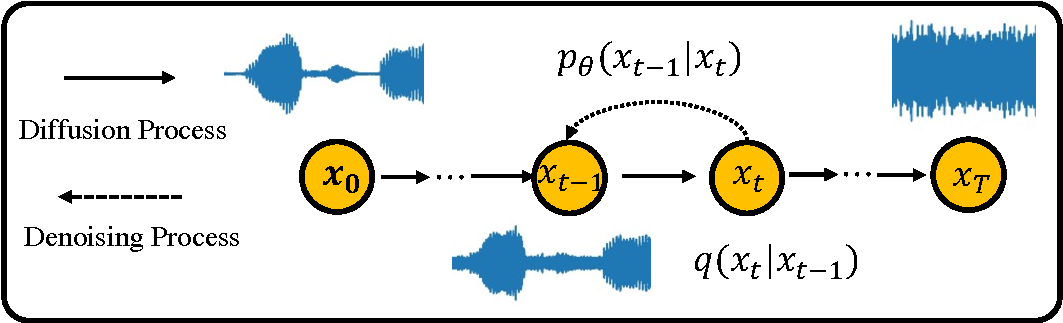
\includegraphics[width=0.45\textwidth]{Figures/process.pdf}
    % \vspace{-1mm}
   \caption{Conditional Diffusion Model for Speech Synthesis} 
%   \vspace{-2mm}
    \label{fig:process}
  \end{figure}

\section{Related Works}

Text-to-speech (TTS) systems aim to synthesize raw speech waveforms from given text. In recent years, Neural network based TTS~\cite{ren2020fastspeech,kim2020glow,liu2021diffsinger} has made huge progress and attracted a lot of attention in the machine learning and speech community.
% , which typically utilize a two-stage pipeline: 1) Convert input text or phoneme sequences into acoustic features (i.e., mel-spectrogram) 2) Transform these feature to waveforms using a vocoder. 

Neural vocoder plays the most important role in the recent success of speech synthesis, which require diverse receptive field patterns to catch audio dependencies: 1) autoregressive model WaveNet~\cite{oord2016wavenet} requires causal convolutions layers and large filters to increase the receptive field while suffering from slow inference speed. 2) Flow-based generative models~\cite{prenger2019waveglow} fully utilize modern parallel computing processors to broaden corresponding receptive fields and speed-up sampling, while they usually achieve a limited sample quality. 3) Generative adversarial networks (GANs)~\cite{jang2021univnet,kong2020hifi} are one of the most dominant deep generative models in audio generation. UnivNet~\cite{jang2021univnet} has demonstrated its success in using local-variable convolution on different waveform intervals, and HIFI-GAN~\cite{kong2020hifi} proposes multi-receptive field fusion (MRF) to model the periodic patterns matters. However, GAN-based models are often difficult to train, collapsing~\cite{creswell2018generative} without carefully selected hyperparameters and regularizers, and showing less sample diversity. 4) Recently proposed diffusion models Diffwave~\cite{kong2020diffwave} and WaveGrad~\cite{chen2020wavegrad} could generate high-quality speech samples, while suffering from a distinct degradation when reducing reverse iterations, making diffusion models difficult to get accelerated. Different from vocoders mentioned above, FastDiff improves the robustness of conditional diffusion model by catching the details of noisy samples at dynamic dependencies, and reduces reverse iterations with predicted noise schedule. The proposed conditional diffuion model allows the high-quality speech synthesis with computational efficiency. 

Another important line of work covers directly waveform generation from text: FastSpeech 2s~\cite{ren2020fastspeech} and VITS~\cite{kim2021conditional} adopt adversarial training process and spectral losses for improving audio quality, while they do not take full advantage of end-to-end training. Recently proposed WaveGrad 2~\cite{chen2021wavegrad} estimates the gradient of the log conditional density of the waveform given a phoneme sequence, but suffers from a large model footprint and slow inference. Unlike all of the aforementioned methods, as highlighted in section~\ref{FastDiff_TTS}, FastDiff-TTS is a fully differentiable and efficient architecture that produces waveforms directly without generating middle features (e.g., spectrograms) explicitly. In additional, our diffuion probabilistic model gets free from hundred or thousands of iterations and enjoy computational efficiency.
